\documentclass[a4paper,11pt]{jsarticle}


% 数式
\usepackage{amsmath,amsfonts}
\usepackage{bm}
\usepackage{physics}
% 画像
\usepackage[dvipdfmx]{graphicx}
\usepackage[hang,small,bf]{caption}
\usepackage[subrefformat=parens]{subcaption}
\captionsetup{compatibility=false}
% ローマ数字
\usepackage{otf}
% 単位
\usepackage{siunitx}
% 表
\usepackage{multirow}
% 化学反応
\usepackage[version=4]{mhchem}


\begin{document}

\title{}
\author{}
\date{\today}
\maketitle

\begin{figure}[htbp]
  \centering
  \begin{minipage}{0.45\linewidth}
    \centering
    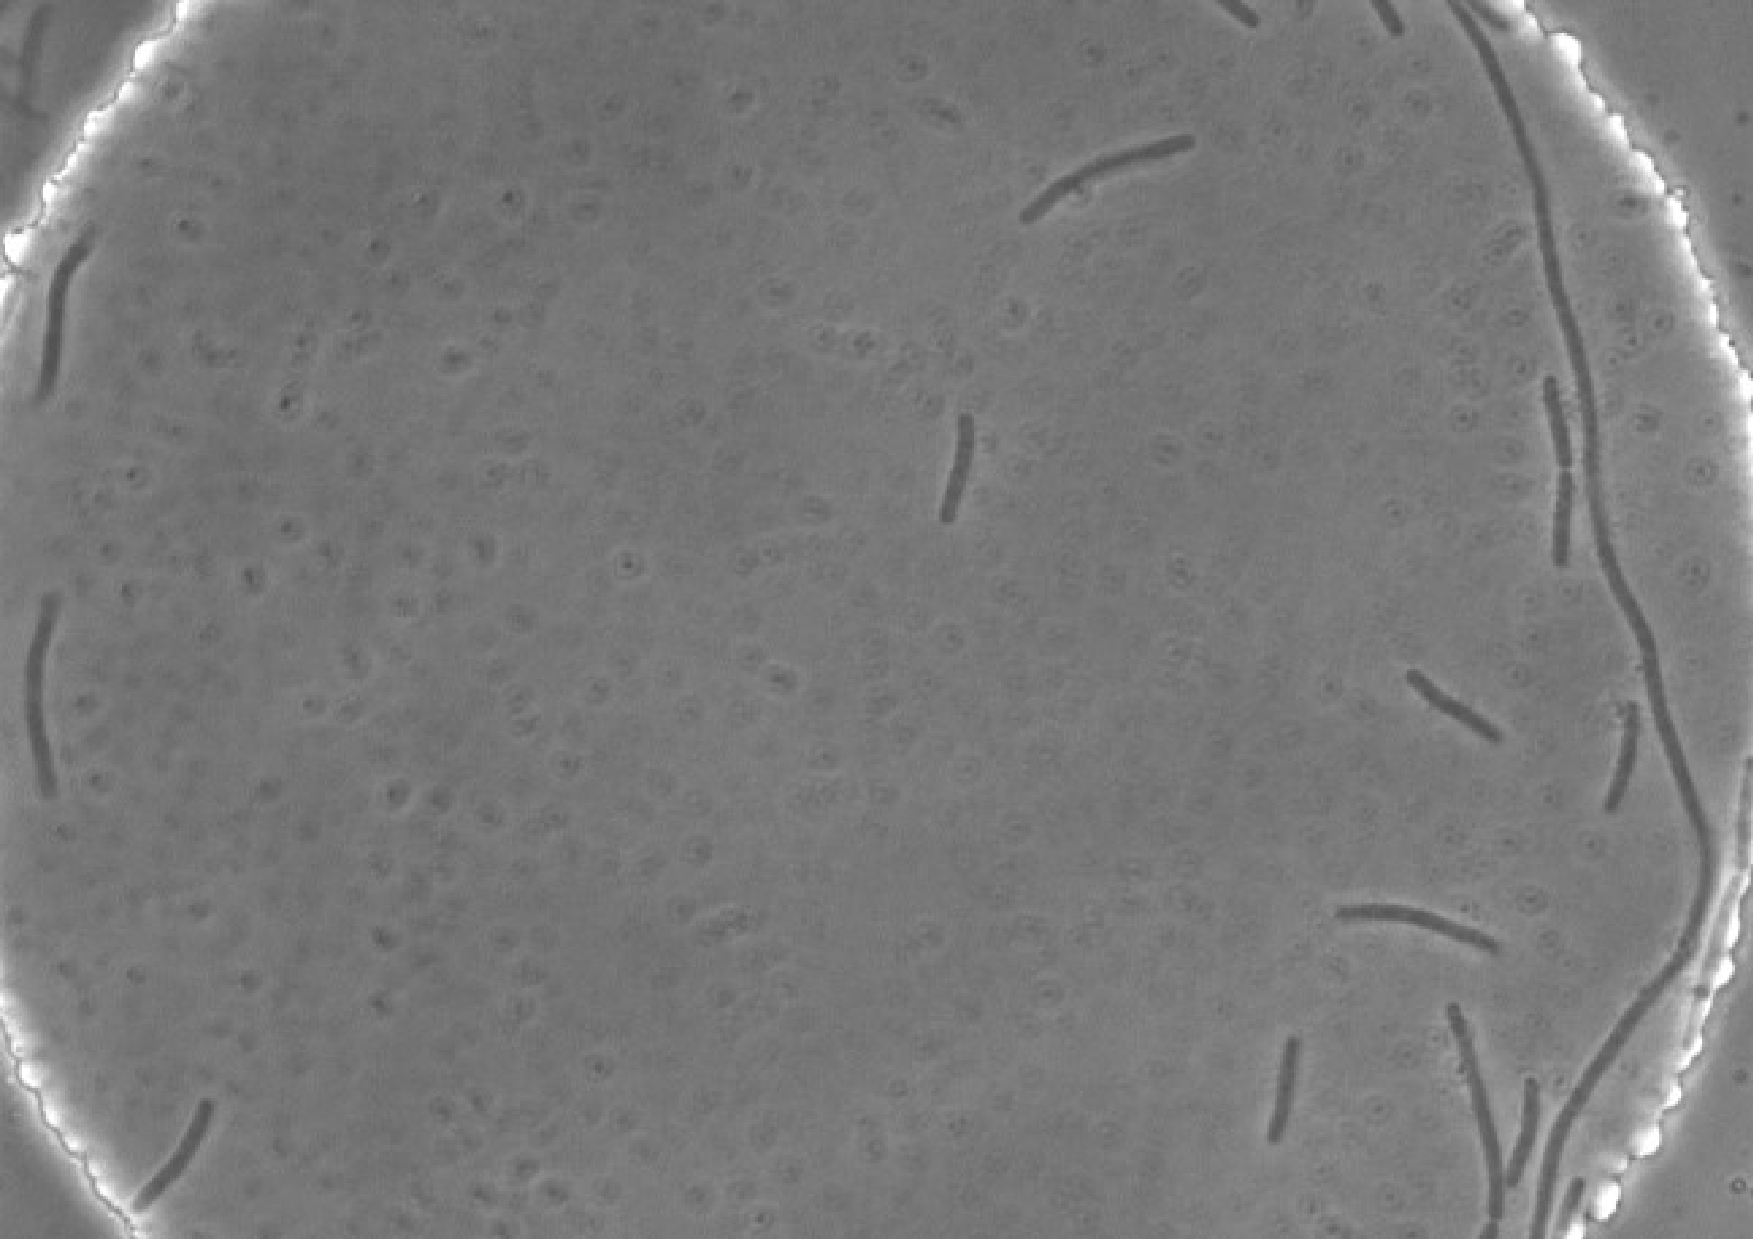
\includegraphics[width=\columnwidth]{Series015_t000000_RAW_ch00.pdf}
    \caption{}
    \label{fig:1}
  \end{minipage}
  \begin{minipage}{0.45\linewidth}
    \centering
    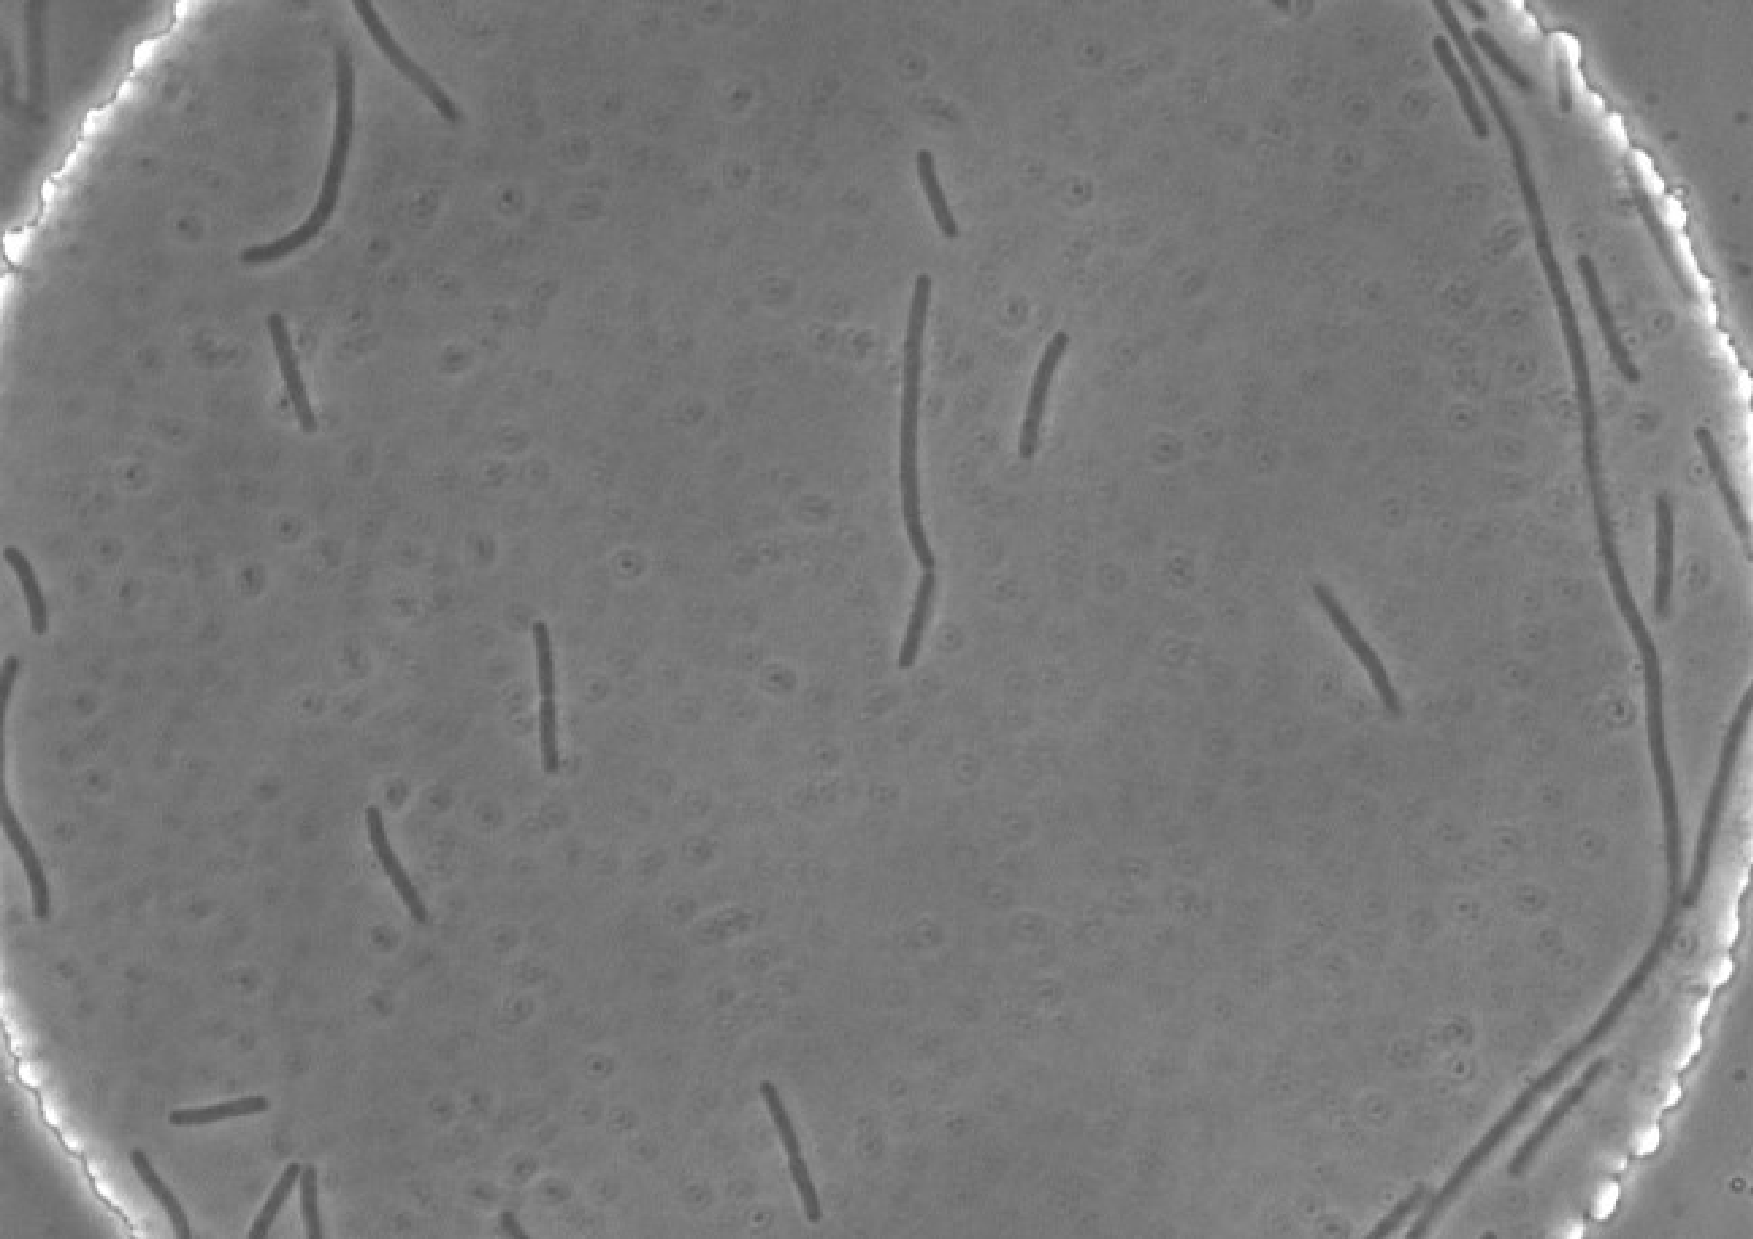
\includegraphics[width=\columnwidth]{Series015_t010000_RAW_ch00.pdf}
    \caption{}
    \label{fig:2}
  \end{minipage}
  \begin{minipage}{0.45\linewidth}
    \centering
    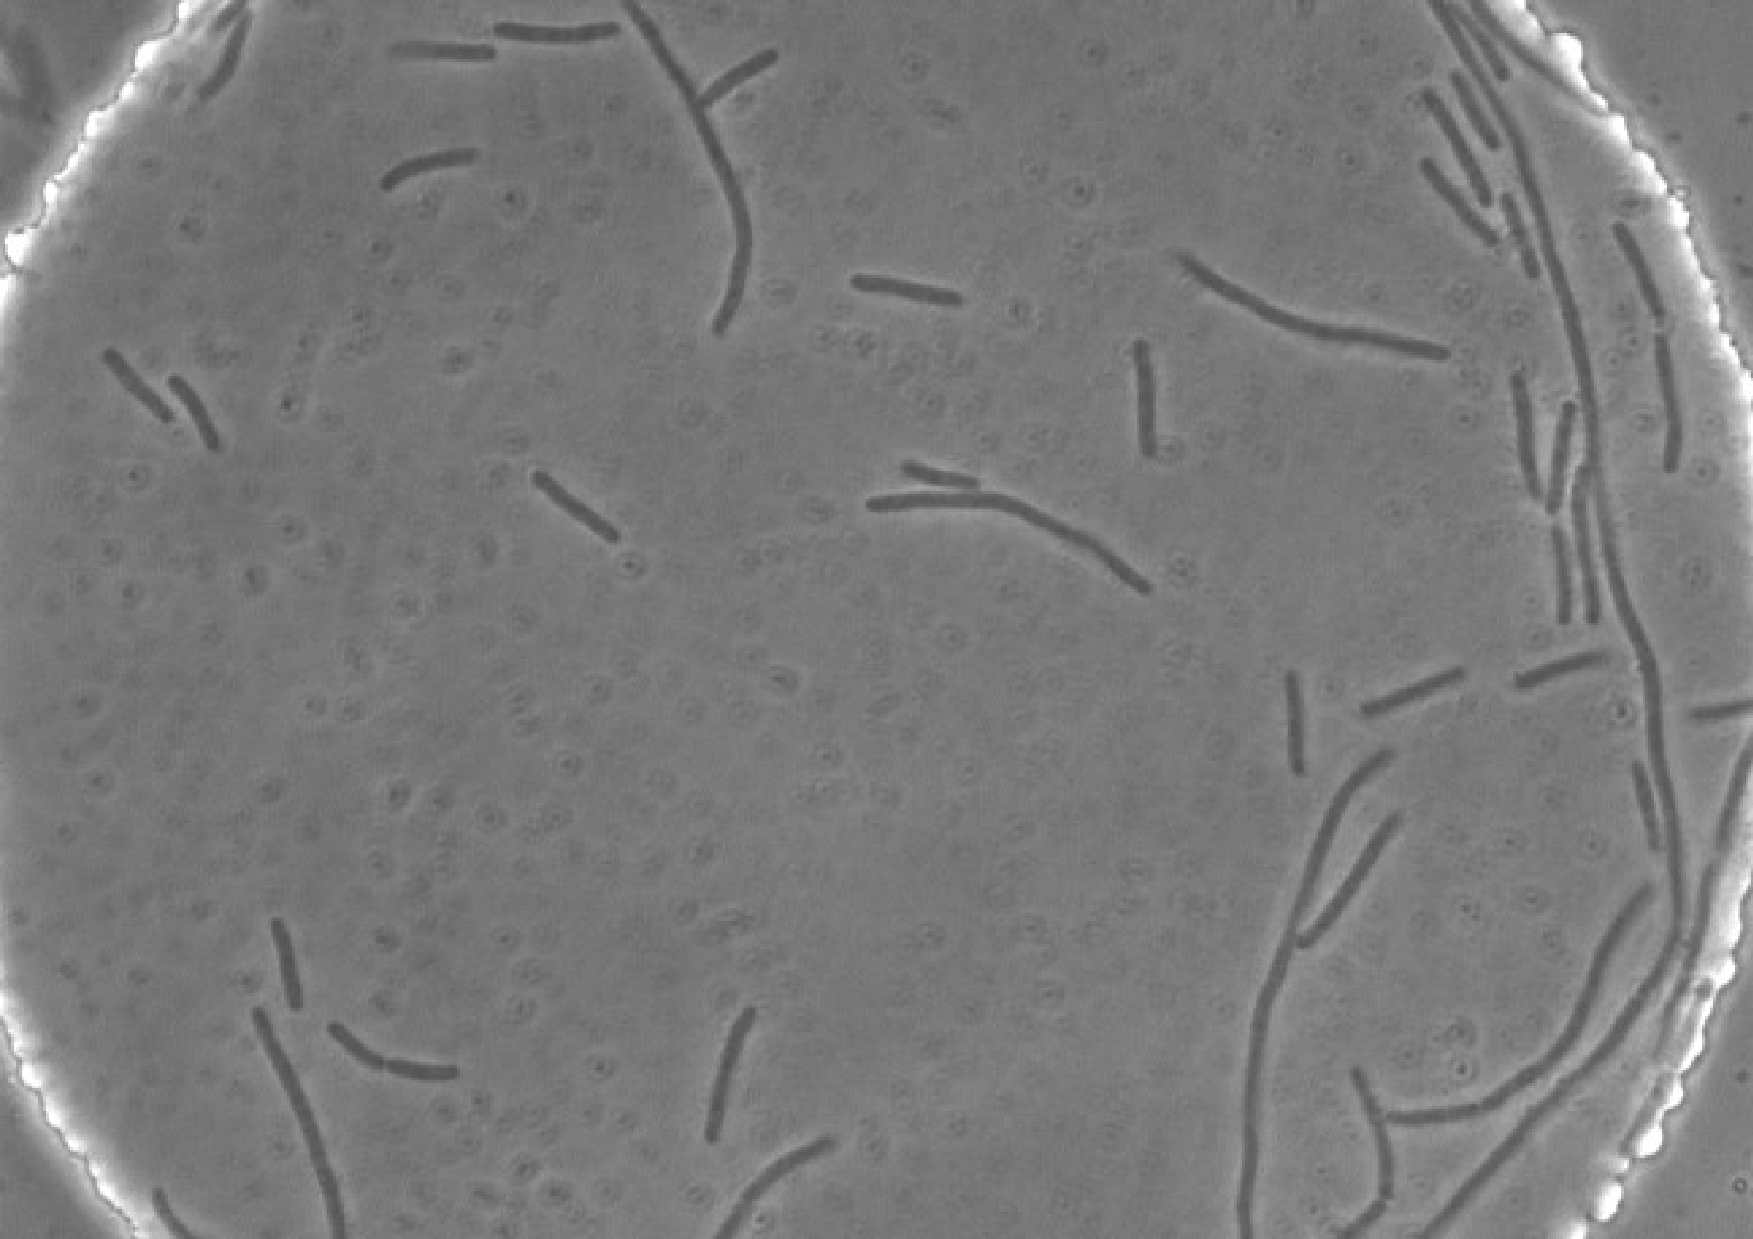
\includegraphics[width=\columnwidth]{Series015_t020000_RAW_ch00.pdf}
    \caption{}
    \label{fig:3}
  \end{minipage}
  \begin{minipage}{0.45\linewidth}
    \centering
    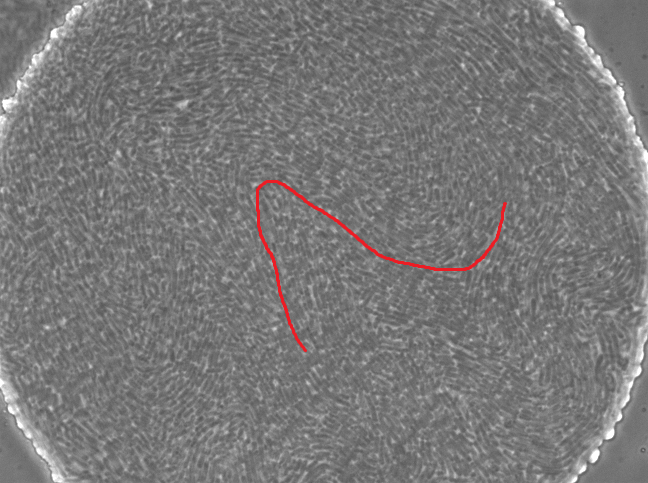
\includegraphics[width=\columnwidth]{Series015_t180000_RAW_ch00.png}
    \caption{}
    \label{fig:4}
  \end{minipage}
\end{figure}

\begin{figure}[htbp]
  \centering
  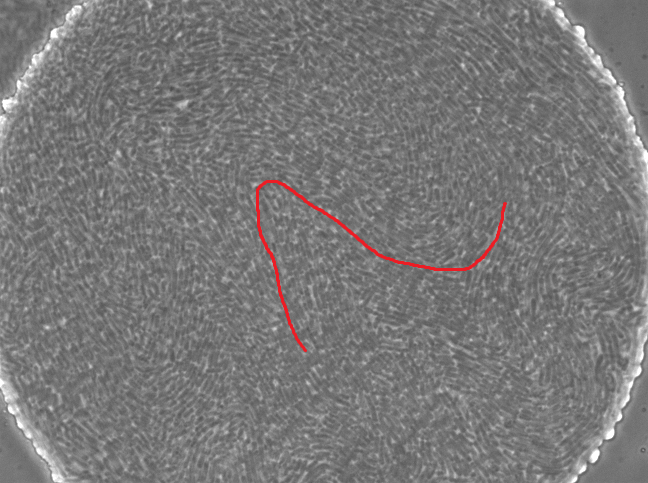
\includegraphics[width=\columnwidth]{Series015_t180000_RAW_ch00.png}
  \caption{}
  \label{fig:}
\end{figure}

\begin{figure}[htbp]
  \centering
  \begin{minipage}{0.45\linewidth}
    \centering
    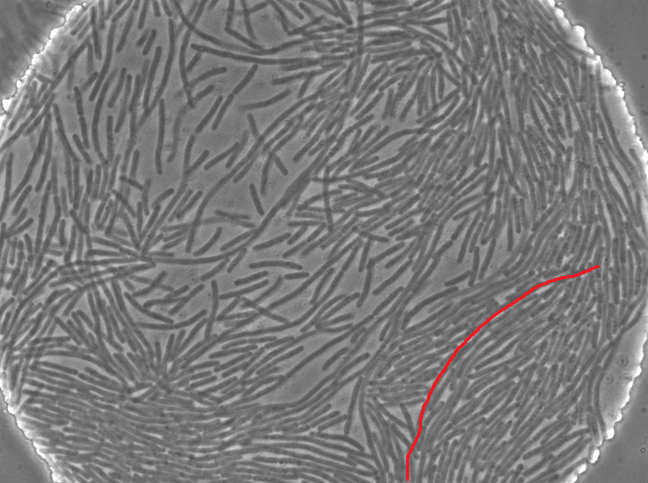
\includegraphics[width=\columnwidth]{Series015_t090000_RAW_ch00.png}
    \subcaption{菌液注入から約後}
    \label{fig:06_1_pt}
  \end{minipage}
  \begin{minipage}{0.45\linewidth}
    \centering
    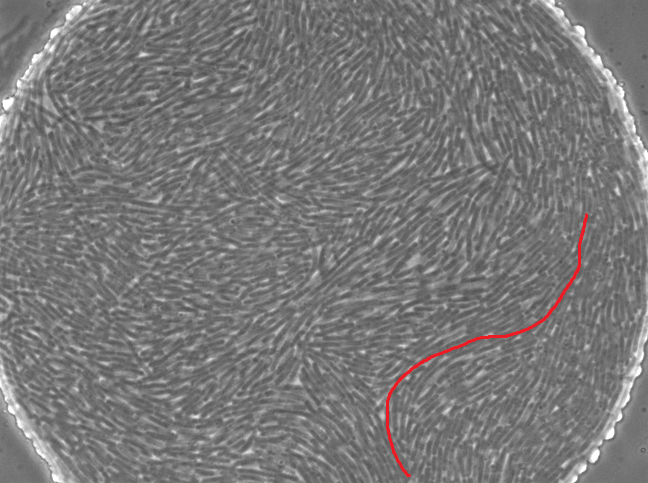
\includegraphics[width=\columnwidth]{Series015_t120000_RAW_ch00.png}
    \subcaption{菌液注入から約後}
    \label{fig:06_2_pt}
  \end{minipage}
  \begin{minipage}{0.45\linewidth}
    \centering
    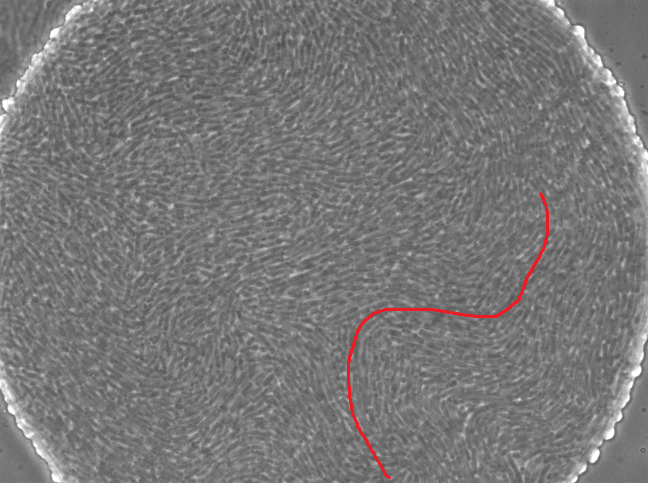
\includegraphics[width=\columnwidth]{Series015_t150000_RAW_ch00.png}
    \subcaption{菌液注入から約後}
    \label{fig:06_3_pt}
  \end{minipage}
  \begin{minipage}{0.45\linewidth}
    \centering
    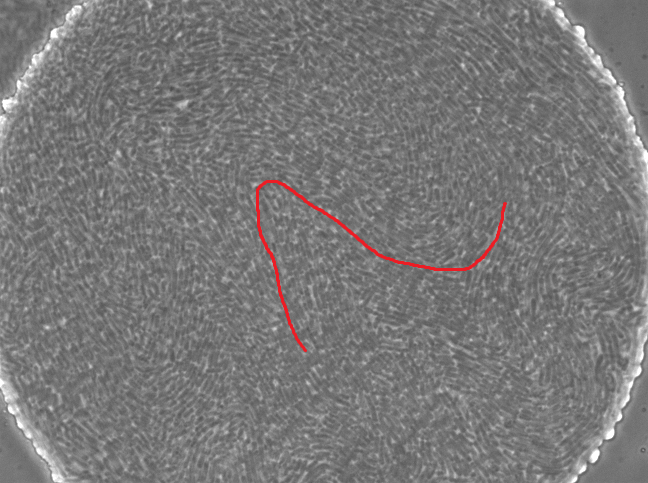
\includegraphics[width=\columnwidth]{Series015_t180000_RAW_ch00.png}
    \subcaption{菌液注入から約後}
    \label{fig:06_4_pt}
  \end{minipage}
  \caption{UU2806を用いた実験の結果.繊維状の個体に対応する場所を赤くマークした.}
\end{figure}

\end{document}